\section{Design \& Implementation}
\label{sec:searchspace_construction}
This section discusses the design and implementation details of our novel method for efficiently constructing large search spaces for GPU auto-tuning. 
We first provide the background and possible approaches to solutions within the context of auto-tuning frameworks in~\cref{subsec:searchspace_construction_context}. 
Following this, \cref{subsec:searchspace_construction_packages} examines various constraint-solving techniques to find a basic approach best suited within the problem context. 
Next, the selected basic approach is optimized in~\cref{subsec:searchspace_construction_improvements}, resulting in a substantially improved search space construction process.
Finally the representation and application of the resulting search space in auto-tuning frameworks is detailed in~\cref{subsec:searchspace_construction_searchspace_object}. 
% 3.1: hoe past dit search space construction probleem in de autotuning context? -> we weten wat de uitdagingen zijn
% 3.2: welke oplossing uit de solving-velden is het meest geschikt als basis voor autotuning? -> we hebben een basis
% 3.3: wat voor verbeteringen brengen we aan in die basis-oplossing? -> we hebben onze oplossing
% 3.4: hoe passen we onze oplossing optimaal toe in autotuning frameworks zoals Kernel Tuner? -> we hebben de uitdagingen opgelost

\begin{figure}[htb]
    \centering
    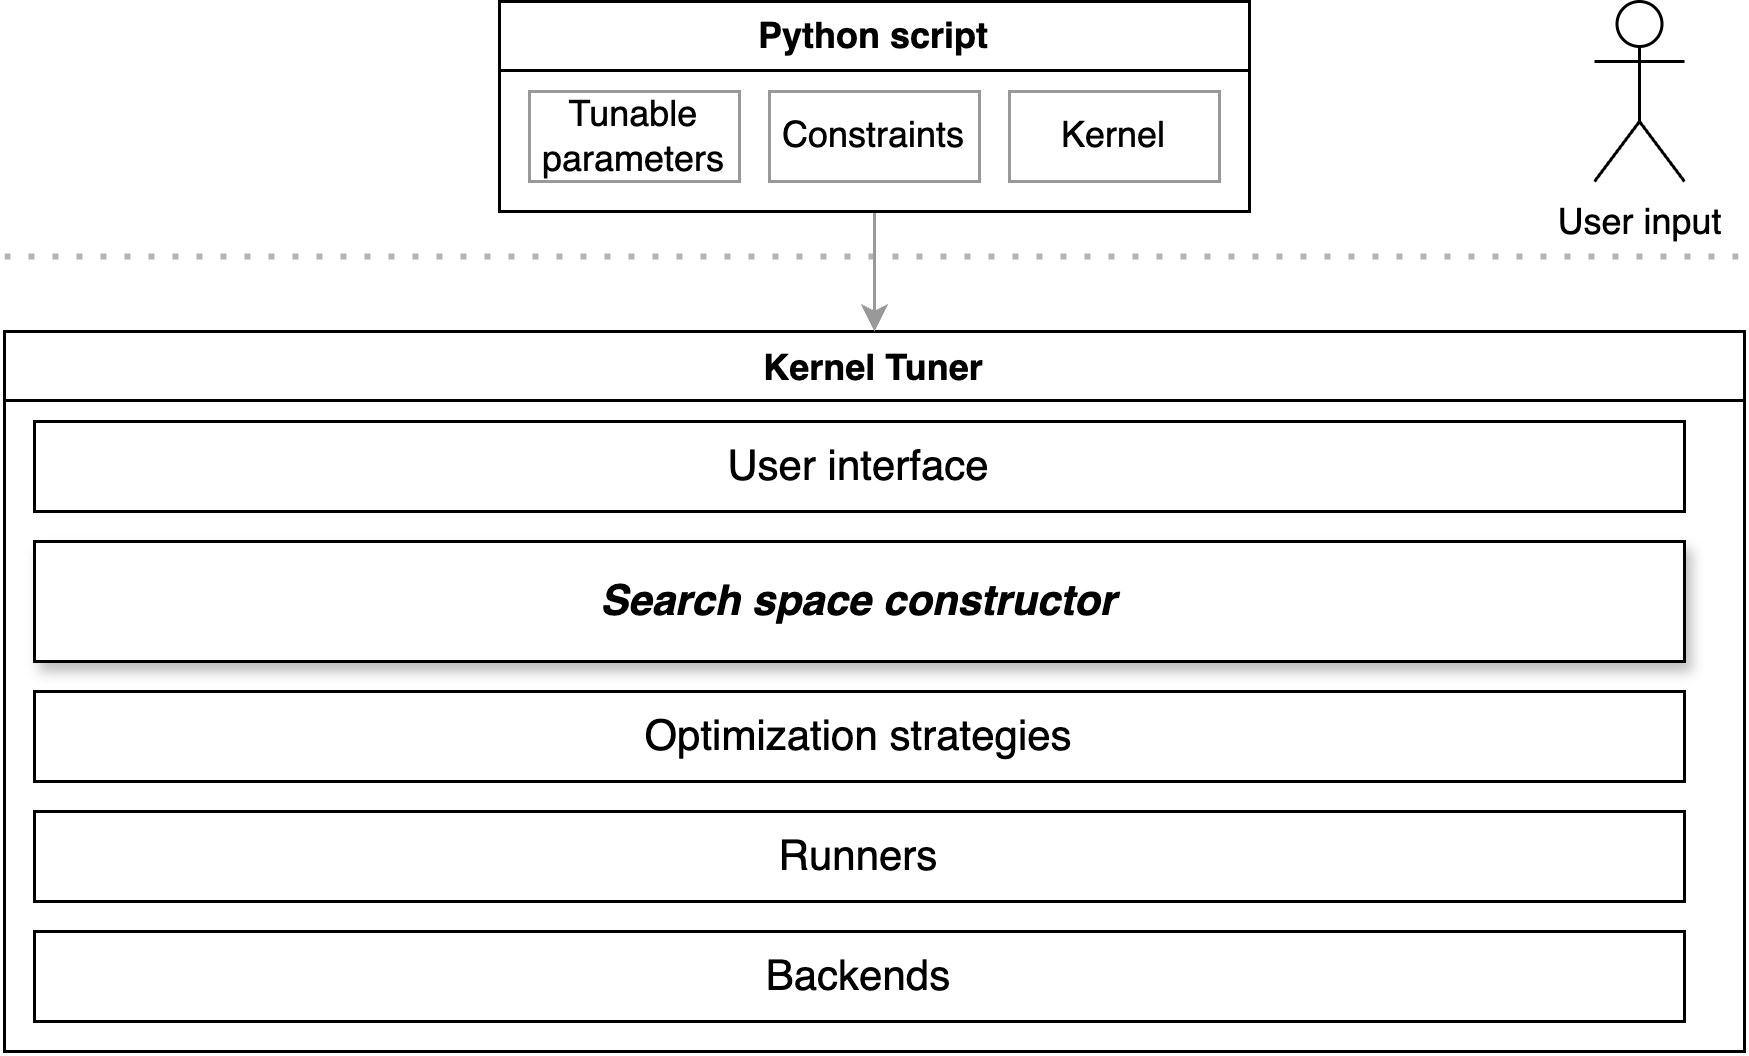
\includegraphics[width=\linewidth]{ics25template/figures/kt_architecture_simplified.png}
    \caption{Abstract Kernel Tuner software architecture.}
    \Description[Kernel Tuner software architecture]{A diagram of the Kernel Tuner software architecture, including the user inputs and external backends.}
    \label{fig:kernel-tuner-architecture}
\end{figure}

\subsection{Problem and Solution Context} \label{subsec:searchspace_construction_context}
To understand the background of the search space construction problem and explore various approaches to solutions in this subsection in an auto-tuning context, we focus on a specific auto-tuning framework.
In \cref{sec:related_work}, we discussed three open-source auto-tuning frameworks that use brute-force search space construction, which suffices for auto-tuning problems that could be manually explored, but can take a substantial amount of time with the large search spaces currently encountered. 
As in this work we aim to provide a generic efficient solution for the construction of large search spaces for auto-tuning, we implement this in the most actively developed of these three open-source auto-tuning frameworks, Kernel Tuner, to demonstrate our novel method.

Kernel Tuner is an external framework for developers to benchmark and optimize GPU kernels in isolation, which can be used with applications in any host programming language. 
The abstract software architecture of Kernel Tuner is shown in Figure~\ref{fig:kernel-tuner-architecture}. Users of Kernel Tuner create a small Python script that points to the kernel and describes both the tunable parameters and any constraints (referred to as {\em restrictions} by Kernel Tuner) to filter out invalid combinations of parameter values. 
There are also various optional settings that users can specify, such as derived metrics to be computed, the optimization objective to use, which optimization algorithm to use, and hyperparameters to the optimization algorithm of choice. 

Search space construction is the first step towards auto-tuning any function or application, preceding the search through the myriad of configurations or code variants. This is apparent from \cref{fig:kernel-tuner-architecture}, where the modular structure of Kernel Tuner is shown, with processing flowing generally from the top (user input), through the search space constructor, to the strategies (optimization algorithms) that determine the next configuration to evaluate, to the runners that prepare the evaluation, and the backends that compile and execute the kernel. After execution, the process flows back up in the diagram, either to the strategies to determine the next configuration based on the new result and repeat the process, or by reporting the best configuration found to the user. 

% In this section, we explore a fundamental change to the search space construction process, leading to a speedup of several orders of magnitude.     

% This section examines the performance improvements that have been made 
% As auto-tuning tools become more efficient, increasingly larger search spaces become feasible. As a result of this development, the efficiency with which all valid configurations (configurations that meet constraints specified by the user) are found, can have a significant impact on the total tuning time. 
% This section examines performance improvements for search space construction in Kernel Tuner. 
% This section discusses the performance improvements in Kernel Tuner for search space construction, and compares this performance to the state of the art in auto-tuning search space construction: Auto-Tuning Framework (ATF) \cite{raschATFGenericAutoTuning2017}. 

In this work, we will focus on the \textit{search space constructor} part of \cref{fig:kernel-tuner-architecture}, as with possibly billions of code variants to enumerate in a high-dimensional space, where user-defined constraints cut out parts of the space that are considered invalid, constructing the search space can become a bottleneck at the start of the tuning process. 
In GPU auto-tuning, the Cartesian product of the tunable parameters, that is, the collection of all possible combinations of all parameter values, tends to contain many configurations that are not valid. For example, because the product of the thread block sizes can not be larger than some hardware limitation, or because some combination of parameter values would lead to incorrect results in the kernel. To filter out such configurations, the user can specify constraints on certain combinations of tunable parameter values. 

The most straight-forward solution is brute force: generate all the combinations of parameter values and filter out combinations based on the user-specified constraints, leaving only valid configurations. This is reasonable for small search spaces but becomes increasingly time-consuming as the search space size and number of constraints increase.
Hence, to improve performance on large search spaces, the search space must be constructed more efficiently. 

One approach could be to resolve the constraints dynamically, either by only checking the constraints of combinations suggested by the optimization strategy before executing kernel configurations, or by resolving the search space in parallel while executing. 
However, these dynamic approaches pose problems. 
If we take the approach of only checking combinations suggested by the strategy, in tuning problems with sparse search spaces (where the vast majority of combinations of parameter values are not valid configurations), a substantial amount of time would be spent on finding any valid configuration as for each combination the optimization strategy needs to be consulted and the combination checked against the constraints. 
This problem is exacerbated by the fact that during the tuning process, the number of valid non-executed configurations decreases. To illustrate this, in the case of a random search on a search space of 100 valid configurations in a search space where 99\% is invalid (10000 combinations) and configurations are taken from the search space once executed, the expected number of attempts required to find a valid first configuration is 100. % 1/(100/10000)
However, the expected number of attempts required to find the fiftyfirst valid configuration is 199, and the sum of expected attempts required from the first to the fiftyfirst valid configuration is over 7000 - over two-thirds of the total Cartesian size of the space. % 1/(50/(10000-(-50+100))=199
While this can be mitigated by keeping track of all attempted combinations, this by itself produces a large memory footprint. 
Moreover, dynamic resolution can skew initial sampling and strategies, as the knowledge of the constraints is not fully incorporated in the search. % This can be as illustrated as follows: given a search space with two parameters, $X$ and $Y$, both with values $(2, 3, 4)$, this results in nine possible combinations of these parameter values. Adding the constraint $X > Y$ leaves three valid configurations: $((3,2),(4,2),(4,3))$. If want to take a random configuration from this search space, these three configurations ideally have an equal chance of being drawn. However, if we have previously drawn the 
% The final problem with dynamic search space resolution is particularly 

An example of a dynamic approach to search space resolution in auto-tuning is the chain-of-tree approach used by ATF~\cite{ATF} as described in \cref{subsec:related_work_software_autotuning}. While this is efficient for search spaces where the vast majority of possible combinations are invalid, individual constraints may only use a small subset of all the parameters to achieve this efficiency. 
In addition, search space characteristics such as the true parameter bounds, which can help optimization algorithms navigate the space more efficiently and enable fairly distributed sampling methods such as Latin Hypercube Sampling~\cite{willemsenBayesianOptimizationAutotuning2021}, are not resolved with the dynamic approach. Furthermore, randomized sampling is inherently biased to the sparser parts of the tree, although this has been addressed by BaCO~\cite{BaCO2024}. Moreover, selecting neighbors of configurations as extensively used by various optimization algorithms in Kernel Tuner is potentially expensive. 

Instead, we aim to fully resolve the search space before starting the tuning process, with a minimal impact on the total execution time, to incorporate the full information of the search space in the initial sampling and search strategies. 

\subsection{Using Constraint Solvers in Auto-tuning} \label{subsec:searchspace_construction_packages}
In general, this type of problem, where parameter values and constraints are resolved to valid combinations, can be encoded as a Boolean Satisfiability Problem (SAT) \cite{biereHandbookSatisfiabilityVolume2009}, Satisfiability Modulo Theories (SMT) \cite{barrett2008satisfiability}, or Constraint-Satisfaction Problem (CSP) \cite{brailsfordConstraintSatisfactionProblems1999}. At the time of writing, several frameworks are readily available as Python packages that have implemented solvers for these types of problems: \textit{CSP-solver} \cite{maniCSPSolverLibrarySolve}, \textit{Google ORTOOLS} \cite{llcOrtoolsGoogleORTools}, \textit{PicoSAT} \cite{schnellPycosatBindingsPicosat}, \textit{CPMpy} \cite{gunsCPMPy}, \textit{PyChoco} \cite{prudhommePychocoPythonBindings}, \textit{SATisPy} \cite{laszloSatispyInterfaceSAT}, \textit{PySMT} \cite{teamPySMTSolveragnosticLibrary}, \textit{python-constraint} \cite{niemeyerPythonconstraintPythonconstraintModule}. 
Nevertheless, not all of these frameworks can be applied to auto-tuning; they have their limitations in how expressive and efficient they are. In general, the SAT, SMT, and CSP problem types mentioned serve different purposes, owing to their different origins. SAT solvers are generally most efficient, at the cost of expressivity, as they are highly optimized for propositional logic problems. SMT solvers allow for non-integer finite domains such as floating-point numbers, strings, and lists, and as such are more expressive, although not as optimized as SAT solvers. CSP solvers offer high-level abstractions suitable for modeling complex constraints, providing special types such as "all-different" \cite{stojadinovicMeSATMultipleEncodings2014}, which are otherwise difficult to efficiently express, making them ideal for complex combinatorial constraints. 

In auto-tuning, the constraint problem consists of a set of named parameters, each parameter having a finite list of possible values, usually numeric but also strings or other types. As such, SMT and CSP solvers are the best fit in this case, % discarding \textit{ORTOOLS}, \textit{PicoSAT}, \textit{CPMpy}, and \textit{SATisPy} as these provide or expose SAT solvers. That leaves 
leaving \textit{CSP-solver}, \textit{PyChoco}, \textit{PySMT}, and \textit{python-constraint}. In addition, there are practical considerations when it comes to choosing a solver; \textit{PyChoco} is in beta at the time of writing and requires building from source, and \textit{PySMT} requires manual steps to install actual solvers, making it cumbersome to deploy as a dependency within a framework. Various solvers, such as \textit{CSP-solver} and the Microsoft Z3 solver in \textit{PySMT}, aim to find any solution, rather than all solutions, as required in the case of auto-tuning. To obtain all solutions, such solvers must iteratively find a solution, add this solution as an additional constraint, and look for the next solution until there are no solutions left \cite{bjornerProgrammingZ32019}. If there are many solutions, as is commonly the case with auto-tuning problems, this can have a substantial impact on performance. 

Hence, we focus on \textit{python-constraint}, as this is a CSP-based Python package with built-in support to find all solutions. Initially developed by Gustavo Niemeyer and afterwards maintained by Sébastien Celles, the \textit{python-constraint} package was first released in 2005. The more than 22000 weekly downloads\footnote{\url{https://pypistats.org/packages/python-constraint}} at the time of writing indicate that the package has a substantial user base. 

\subsection{Implementation of Optimizations} \label{subsec:searchspace_construction_improvements}
Based on \cref{subsec:searchspace_construction_packages}, we use the \textit{python-constraint} package as a basis for our implementation. To obtain the level of performance required to construct auto-tuning search spaces efficiently, we implement several key improvements in various areas: algorithmically (\cref{subsubsec:searchspace_construction_improvements_algorithm}), by extending and improving constraints (\cref{subsubsec:searchspace_construction_improvements_constraints}), by introducing parsing (\cref{subsubsec:searchspace_construction_improvements_parser}), by providing tailored output formats (\cref{subsubsec:searchspace_construction_improvements_output_formats}), and finally engineering (\cref{subsubsec:searchspace_construction_improvements_engineering}). 

\subsubsection{Algorithm} \label{subsubsec:searchspace_construction_improvements_algorithm}
We select and optimize a backtracking solver optimized for finding all solutions rather than any solution. This algorithm maintains a dictionary of variable assignments and uses a stack-based approach to implement iterative backtracking, avoiding recursive function calls. Variables are selected dynamically using a combination of the Minimum Remaining Values (MRV) and Degree heuristics, prioritizing those with fewer remaining values and higher connectivity. For each selected variable, domain values are checked against the constraints. If a constraint is violated, the algorithm backtracks by restoring previous states from a queue until all possibilities are explored. 
We have optimized this algorithm by sorting the variables on the number of internal constraints, making it faster to find unassigned variables, and by reducing the number of sorts required. 
By systematically iterating through variable assignments and leveraging heuristics, the algorithm efficiently constructs all valid solutions while minimizing unnecessary exploration. 

\subsubsection{Constraints} \label{subsubsec:searchspace_construction_improvements_constraints}
We expand and improve built-in specific constraints to optimize operations that are commonly used. 
Commonly used operations allow for increased efficiency over generic functions by applying knowledge of the operation. For example, given a constraint where $p \cdot q > 0$, we know to ignore all cases where $(p \leq 0) \xor (q \leq 0)$. 
We added \textit{MaxProduct} and \textit{MinProduct} constraints as they are commonly used in auto-tuning constraints (e.g. a maximum product of block sizes due to hardware limits). We also rewrote and added preprocessing steps to the \textit{Function}, \textit{MaxSum} and \textit{MaxProduct} constraints.  
The \textit{Function} constraint is particularly interesting for optimization, as it is both a computationally expensive constraint due to its generality and a common occurrence as it is used wherever the more specific constraints do not apply. We have optimized this by employing function rewriting and dynamic runtime compilation, as the one-off expense of compilation to bytecode is offset by the potentially many times a \textit{Function} constraint is executed. % Bytecode is a low-level representation of code specific to the Python virtual machine (PVM), which executes the bytecode to perform the desired operations.
% Given that the \textit{Function} constraint is both a common occurrence as it is used wherever the more specific constraints do not apply and a generally more computationally expensive constraint due to its generality and the fact that it may call on external functions, it has been optimized in particular by employing function rewriting and runtime compilation. 

\subsubsection{Parser} \label{subsubsec:searchspace_construction_improvements_parser}
We introduce a parser for constraints written in string format, which has three important benefits: to apply the more efficient specific constraints instead of generic functions where possible, to break down constraints into the smallest subsets of variables, thereby aiding the constraints solver, and to provide all of this without requiring users to write their constraints in a complex format that requires understanding how the solvers work. 

To address the latter benefit first, most solvers and tuners require specific function calls or a form of domain-specific language when defining the constraints (as will be encountered in \cref{subsec:evaluation_compared_frameworks}). However, as opposed to the users of CSP-solvers, auto-tuning users are generally not aware of the search space construction process and the specific constraints available that result in efficient resolution of the search space. 
Instead, we provide users the option to write their constraints in Python-evaluable string format, which is then automatically optimized by parsing. 
This usage of Python-evaluable strings has various benefits, as they are both familiar to the user as Python is already the interface language, and rewritable by our parser, allowing the application of specific constraints instead of generic functions and the decomposition of constraints into subsets. 

In particular, the automatic reduction of constraints can be important in scalability and efficiency in practice, as users unfamiliar with the intrinsics of constraint solving, such as the users of auto-tuning frameworks, might write sub-optimal constraints in practice. 
For example, consider the constraint $3 \leq X \cdot Y < 9 \leq Z$, where \textit{X}, \textit{Y}, and \textit{Z} are tunable parameters with numerical values. 
Constraints can not be evaluated until values for the involved parameters are at least partially resolved, resulting in subpar performance in the case of compound statements like the given example, as it depends on three parameters as-is. 
This can be improved by automatically breaking down the constraint into multiple constraints with fewer involved variables where possible. 
For the given example this can be [$3 \leq X \cdot Y$, $X \cdot Y < 9 $, $9 \leq Z$], which allows partially resolved values for either \textit{X}, \textit{Y}, or \textit{Z} to be enough to discard configurations not meeting the constraint earlier in the construction process. 
In addition, this automatic reduction enables the application of specific constraints, as is the case with the example, which can be represented with specific constraints as \lstinline{[(MinProd(3), [x,y]), (MaxProd(9-1), [x,y]), (MinProd(9), [z])]}. As discussed in \cref{subsubsec:searchspace_construction_improvements_constraints}, application of specific constraints can preemptively exclude values through preprocessing, resulting in an even more efficient construction. 

\subsubsection{Output Formats} \label{subsubsec:searchspace_construction_improvements_output_formats}
We implement various output formats to avoid expensive rearrangements to different formats. 
Expensive rearrangement of the structure in which solutions are output by the solver is mitigated by providing output formats that are close to the internal representation, further described in \cref{subsec:searchspace_construction_searchspace_object}.

\subsubsection{Employing C-extensions} \label{subsubsec:searchspace_construction_improvements_engineering}
In general, C and similar languages outperform Python in terms of execution speed~\cite{pythonVSC,comparingSixLanguages}. To attain this level of performance without losing the flexibility and user-friendliness of Python~\cite{pythonVSC++usability}, we employ C-extensions. 
We transpile the codebase from Python to C-code using Cython~\cite{behnelCythonBestBoth2011}, which is then compiled into Python-importable C-extensions. 
We added type hints where possible to aid in compilation. 
Binaries are precompiled for Linux, macOS, and Windows on the supported Python versions (3.9 through 3.13 as of this writing). \\

While the improvements detailed in \cref{subsubsec:searchspace_construction_improvements_algorithm,subsubsec:searchspace_construction_improvements_constraints,subsubsec:searchspace_construction_improvements_parser,subsubsec:searchspace_construction_improvements_output_formats,subsubsec:searchspace_construction_improvements_engineering} are specifically intended to obtain the level of performance required to construct auto-tuning search spaces efficiently, they are generally applicable to any CSP problem. 
Our optimizations have been approved in the main branch of \textit{python-constraint}, benefitting all users of the package and the community. 

\subsection{Search space Representation} \label{subsec:searchspace_construction_searchspace_object}
With the efficient construction of search spaces implemented in \textit{python-constraint}, we consider how this is represented and applied in auto-tuning frameworks in practice to achieve a comprehensive approach. 

As per \cref{subsec:searchspace_construction_context}, after the search space construction, the optimization algorithms use the information obtained in the construction step to select configurations.
Instances of this are obtaining the true bounds of the search space to use balanced initial sampling methods or the selection of valid neighbors that have not been evaluated yet. 
As these type of operations are commonly used in auto-tuning, it can be useful to provide an abstract representation of the search space that implements these operations, providing various views and mappings on the configurations in the search space. 

We have implemented this in Kernel Tuner as the \textit{SearchSpace} class, which takes the tunable parameters and constraints based on the the user specification, constructs the search space using \textit{python-constraint}, and provides various representations and operations on the resulting search space.  
The \textit{SearchSpace} class has multiple internal representations for varying purposes, such as hash- and index-based for efficient lookups. Externally it provides a single interface for all search space-related operations, which in contrast to the initial situation where strategies would implement these operations individually, enables reuse in a modular architecture. 
For example, the mutation step in the \textit{genetic algorithms} optimization strategy requires selecting only valid neighbors within a certain Hamming distance. This, along with other neighbor selection algorithms, is implemented in the \textit{SearchSpace} class and can be indexed before running the algorithm, improving overall performance. 

While we focus on an optimized method for search space construction in auto-tuning, resulting in a generically applicable search space constructor, considering the wider context results in a comprehensive method for search space representations and operations. 
% Various other operations commonly used by the optimization algorithms have been efficiently implemented in this \textit{SearchSpace} class, such as 

% All of these changes are evaluated in synthetic and real-world tests in \Cref{sec:evaluation}. 

% To further improve the performance of \textit{python-constraint} in general and for auto-tuning search spaces specifically, we made the following additional improvements:
% \begin{itemize}
%     \item Cythonization of the codebase. This involves transpiling from Python to C-code with Cython \cite{behnelCythonBestBoth2011}, which is then compiled to Python-importable C-extensions. We added type-hints where possible to aid compilation.
%     \item Expanded and improved built-in constraints. Commonly used operations allow for increased efficiency over generic functions by applying knowledge of the operation. For example, given a restriction where $p \cdot q > 0$, if we have a minimum product constraint specified we know to ignore all cases where $p \leq 0 \lor q \leq 0$. Hence we added \textit{MaxProduct} and \textit{MinProduct} constraints as they are commonly used in auto-tuning restrictions (e.g. a maximum product of block sizes due to hardware limits). We rewrote and added pre-processing steps to the \textit{Function}, \textit{MaxSum} and \textit{MaxProduct} constraints. 
%     \item Automatic reduction and differentiation. On the Kernel Tuner side, we added a parser from restrictions written in string format with two goals: to apply the more efficient built-in constraints instead of generic functions where possible, and to break a restriction down into the smallest subset of variables, as this aids the constraints solver. 
%     \item Improved general efficiency. Several operations were taken from the inner loops of the implemented backtracking algorithm. We added new output formats to avoid expensive rearrangements to different formats. 
% \end{itemize}
% Additionally, the reliability was improved by increasing the test coverage. We improved the maintainability by adding automated workflows for testing, building, documentation, and publishing. 
% The result of these optimizations, compared against brute-force, standard \textit{python-constraint} and the state of the art in auto-tuning search space construction is seen in \Cref{subsec:evaluation_search space}. 
